\section{The Particle Flow Algorithm}


The information available from all CMS subdetectors is employed in the particle-flow (PF) algorithm \cite{CMS:2009nxa,CMS:2010byl} to identify and reconstruct individual particles in the event, namely muons, electrons, photons, and charged and neutral hadrons. These particles are used to reconstruct jets, \hadtau candidates, and the vector imbalance in transverse momentum in the event, referred to as \ptvecmiss, as well as to quantify the isolation of leptons. 

\subsection{Electrons reconstruction}
Electrons are reconstructed by matching tracks in the inner detector with energy depositions in the ECAL \cite{CMS:2009nxa,Baffioni2007}. The tracks of electron candidates are reconstructed using a Gaussian sum filter \cite{Adam:2005bya} algorithm, which accounts for the emission of bremsstrahlung photons along the electron trajectory. Energy loss in bremsstrahlung is reconstructed by searching for energy depositions in the ECAL located in directions tangential to the electron track. A multivariate approach based on boosted decision trees (BDT) \cite{Hocker:2007ht} is employed for electron identification \cite{1748-0221-10-06-P06005}.

\subsection{Muons reconstruction}

 The identification of muons is based on linking track segments reconstructed in the silicon tracking detector and in the muon system \cite{Chatrchyan:2012xi}. The matching between track segments is done outside-in, starting from a track in the muon system, and inside-out, starting from a track reconstructed in the inner detector. In case a link can be established, the track parameters are refitted using the combined hits in the inner and outer detectors, with the resulting track referred to as a global muon track. Quality criteria are applied on the multiplicity of hits, on the number of matched segments, and on the fit quality of the global muon track, quantified through a \ensuremath{\chisquare}.

\subsection {The Jet reconstruction}

Jets within the range \ensuremath{|\eta| < 4.7} are reconstructed using the anti-\ensuremath{k_{T}} algorithm \cite{antikt} with a distance parameter of 0.5. As mentioned previously,the particles reconstructed by the PF algorithm are used as input to the jet reconstruction. Reconstructed jets are required not to overlap with identified electrons, muons, or \hadtau within \ensuremath{\deltar < 0.5}, and to pass two levels of jet identification criteria: (i) misidentified jets, mainly generating from calorimeter noise, are rejected by requiring reconstructed jets to pass a set of loose jet identification criteria \cite{CMS:2010xta} and (ii) jets originating from pileup interactions are rejected through an MVA-based jet identification discriminant, based on information about the vertex and energy distribution within the jet \cite{CMS:2013wea}. The energy of reconstructed jets is calibrated as a function of jet \pt and \ensuremath{\eta} \cite{1748-0221-6-11-P11002}. The contribution of pileup to the energy of jets originating from the hard scattering is compensated by determining a median transverse momentum density (\ensuremath{\rho}) for each event, and subtracting the product of (\ensuremath{\rho}) times the area of the jet, computed in the \ensuremath{\eta-\Phi} plane,from there constructed jet \pt \cite{Cacciari:2008gn, Cacciari:2007fd}. Jets originating from the hadronization of b quarks are identified through the combined secondary vertex (CSV) algorithm \cite{Chatrchyan:2012jua}, which exploits observables related to the long lifetime of b hadrons and the higher particle multiplicity and mass of b jets compared to light-quark and gluon jets.

\begin{figure}
	\centering
	\begin{subfigure}{1\textwidth}
		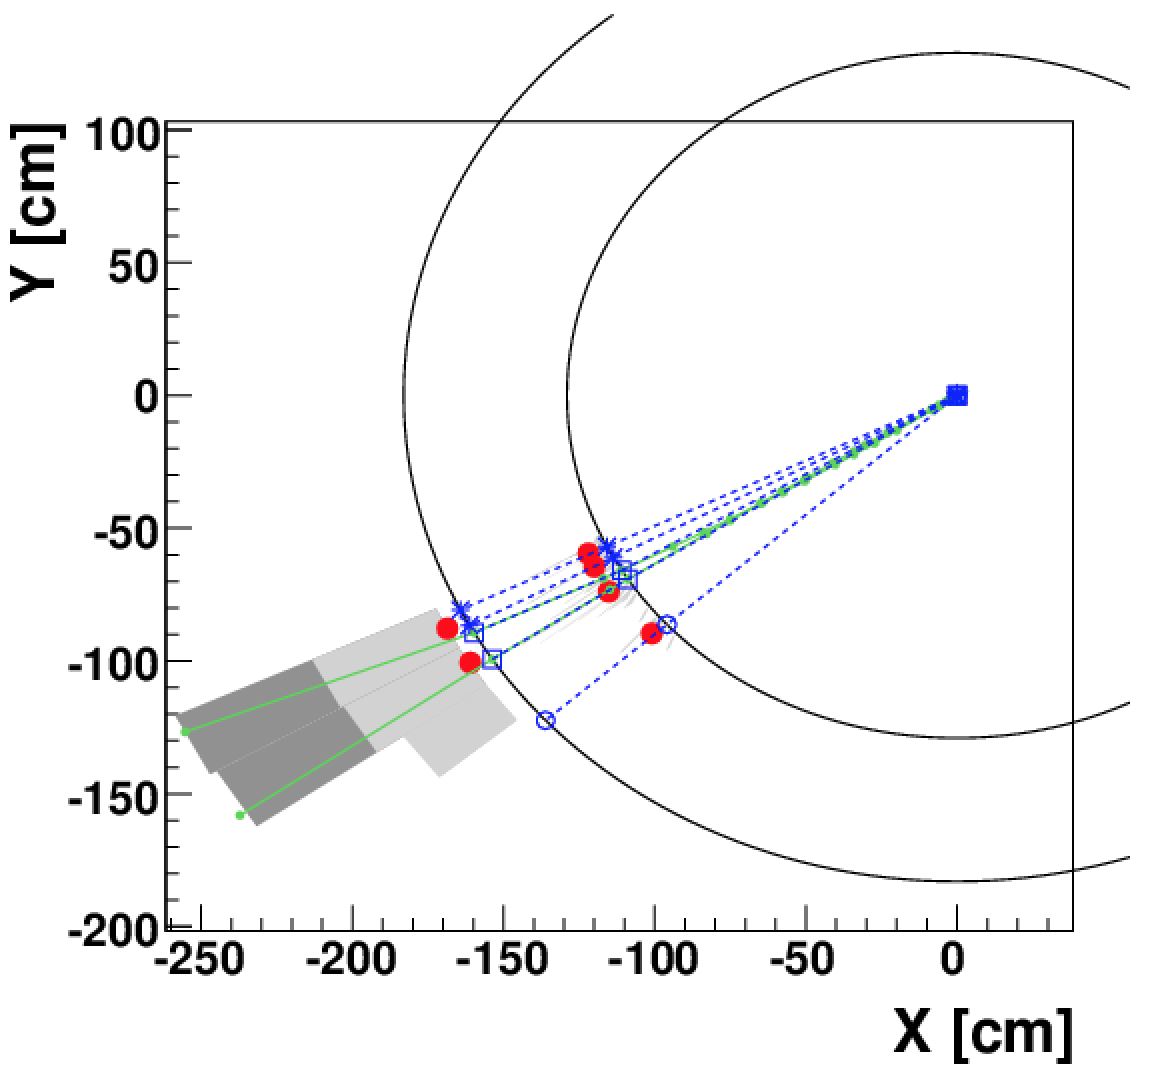
\includegraphics[width=.8\linewidth]{analysis/pics/PF_a.png}
		\caption{The $(x, y)$ view.}
		\label{fig:PF_a}
	\end{subfigure}
	
	\begin{subfigure}{.4\textwidth}
		\centering
		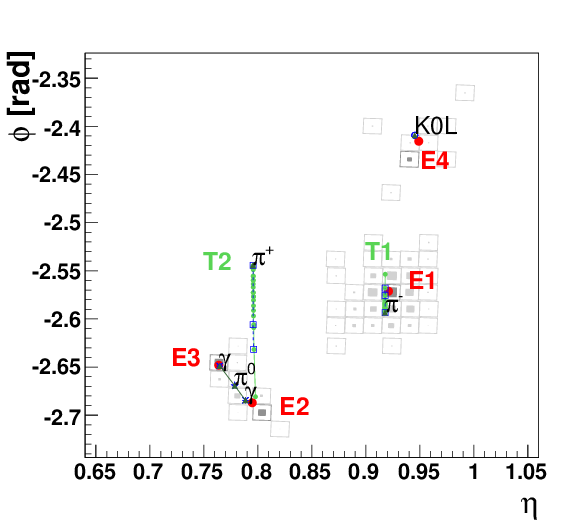
\includegraphics[width=.8\linewidth]{analysis/pics/PF_b.png}
		\caption{The $(\eta,\phi)$ view on ECAL.}
		\label{fig:PF_b}
	\end{subfigure}
	\begin{subfigure}{.4\textwidth}
		\centering
		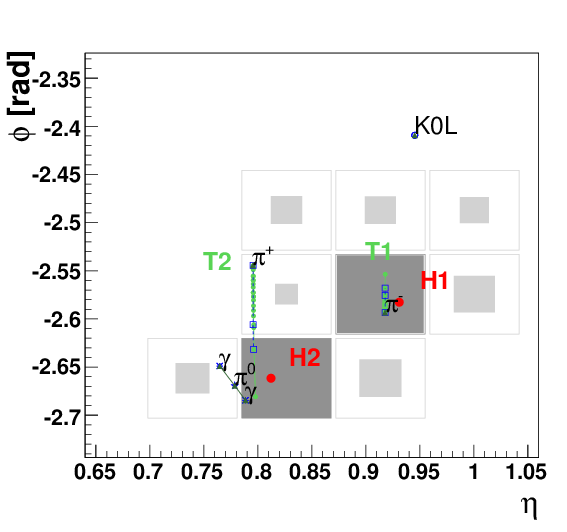
\includegraphics[width=.8\linewidth]{analysis/pics/PF_c.png}
		\caption{The $(\eta,\phi)$ view on HCAL.}
		\label{fig:PF_c}
	\end{subfigure}%
	\caption{An event display of a simple hadronic jet in the $(x, y)$ view (Figure \ref{fig:PF_a}) and in the $(\eta,\phi)$ view, where $\eta$ stands for pseudo-rapidity and $\phi$ for the azimuthal angle, on the ECAL surface (Figure \ref{fig:PF_b}) and the HCAL surface (Figure \ref{fig:PF_c}). (These two surfaces are represented as two circles centred around the interaction point in the first view.) The $K^{0}_{L}$, the $\pi^{-}$ and the two photons from the $\pi^{0}$ decay are detected as four well separated ECAL clusters (Figure \ref{fig:PF_b}). The $\pi^{+}$ leaves no energy in the ECAL. The two charged pions are reconstructed as charged-particle tracks, appearing as vertical solid lines in the $(\eta,\phi)$ views and circular arcs in the $(x, y)$ view. These tracks point towards two HCAL clusters (Figure \ref{fig:PF_c}). In all three views, the cluster positions are represented by dots, the simulated particles by dashed lines, and the position of their impact on the calorimeter surfaces by various open markers.}
	\label{fig:PF_event_display}
\end{figure}

Two algorithms are used to reconstruct \ptvecmiss, the imbalance in transverse momentum in the event, whose magnitude is referred to as \met. The standard algorithm computes the negative vectorial sum of all particle momenta reconstructed using the PF algorithm. In addition, a multivariate regression algorithm \cite{Khachatryan:2014gga} has been developed to reduce the effect of pileup on the resolution in \met. The algorithm utilizes the fact that pileup predominantly produces jets of low \pt, while leptons and high-\pt jets are produced almost exclusively in the hard-scatter. The transverse mass, \mt, of the system constituted by an electron or a muon and \met is used to either select or remove events that are due to W+jets and tt production. 

\clearpage

\section {The Tau Lepton}

The $\tau$ lepton was discovered between 1974 and 1977 by the team under Martin Perl while studying the $e^{+}+e^{-}\longrightarrow e^{\pm}+\mu^{\mp}$. With a mean lifetime of $2.9\times10^{−13}$ s and a mass of 1776.82 \mev \cite{Agashe:2014kda} is the heaviest of the leptons, enough to decay into hadrons, and it does so in about two thirds of the cases, typically into either one or three charged pions or kaons and up to two neutral pions \ensuremath{\pi^{0}}, and one neutrino \ensuremath{\nu_{\tau}}. The \ensuremath{\pi^{0}} meson decays almost exclusively into \ensuremath{\gamma\gamma}. Among all the possible hadronic decays as shown on Table \ref{table:tau_hdecay} the ones called "one-prong", where only one charged hadron is produced, are the most frequent. The $\tau$ decays also leptonically, with a branching ratio of $17\%$ for each channel, via the following decay $\tau\longrightarrow\nu_{\tau}W^{*}\longrightarrow\nu_{\tau}l\nu_{l}$.

\begin{figure}[tbh!]
	\begin{center}	
		\begin{tabular}{ | c | c | c | c |}
			\hline
			Decay Mode & Resonance & Mass [\mev] & BF (\%) \\ \hline
			\hline
			$\tau^{-}\longrightarrow h^{-}\nu_{\tau}$& $\pi$ & 139.6 & 11.6 \\ \hline
			$\tau^{-}\longrightarrow h^{-}\pi^{0}\nu_{\tau}$& $\rho$ & 770 & 26.0 \\ \hline
			%				$\tau^{-}\longrightarrow h^{-}\pi^{0}\pi^{0}\nu_{\tau}$ & $a_{1}$ & 1200 & \\ 10.8 \hline
			$\tau^{-}\longrightarrow h^{-} h^{+} h^{-} \nu_{\tau}$& $a_{1}$& 1200 & 9.8 \\ \hline
			$\tau^{-}\longrightarrow h^{-} h^{+} h^{-} \pi^{0}\nu_{\tau}$& & & 4.8 \\ \hline
			other hadronic channels& & & 1.7 \\ \hline
			\hline
			total & & & 64.8 \\ \hline
			\hline
		\end{tabular}
		\caption{ Hadronic tau decay modes into either one or three charged hadrons h and potential $\pi_{0}$, and the corresponding branching fractions BF. Also shown are the intermediate resonances and their masses, which are used in some of the tau reconstruction algorithms.}
		\label{table:tau_hdecay}
	\end{center}
\end{figure}

\subsection{Algorithm for \hadtau reconstruction and identification}

The \hadtau decays are reconstructed and identified using the hadrons-plus-strips (HPS) algorithm \cite{Chatrchyan:2012zz} and is seeded by jets of \ensuremath{\pt > 14 \gev} and \ensuremath{|\eta| < 2.5}, reconstructed using the anti-\ensuremath{k_{T}} algorithm \cite{antikt} with a distance parameter of 0.5. The algorithm is designed to reconstruct individual decay modes of the \ensuremath{\tau} lepton, taking advantage of the excellent performance of the PF algorithm in reconstructing individual charged and neutral particles.
The reconstruction and identification of \hadtau decays in the HPS algorithm is performed in two steps:

\begin{itemize}
	\item \textbf{Reconstruction:} combinations of charged and neutral particles reconstructed by the PF algorithm that are compatible with specific \hadtau decays are constructed, and the four-momentum, expressed in terms of (\pt, \ensuremath{\eta}, \ensuremath{\phi} , and mass) of τh candidates, is computed.
	
	\item \textbf{Identification:} discriminators that separate \hadtau decays from quark and gluon jets, and from electrons and muons, are computed. This provides a reduction in the jet \ensuremath{\longrightarrow \hadtau}, \ensuremath{e \longrightarrow \hadtau}, and \ensuremath{\mu \longrightarrow \hadtau} misidentification rates.
\end{itemize}

\subsubsection{Identification of decay modes}

Reconstruction of specific \hadtau decay modes requires reconstruction of neutral pions that are present in most of the hadronic \ensuremath{\tau} decays. The high probability for photons originating from \ensuremath{\pi^{0} \longrightarrow \gamma \gamma} decays to convert to \ensuremath{e^{+}e^{-}} pairs within the volume of the CMS tracking detector is taken into account by clustering the photon and electron constituents of the \ensuremath{\tau}-seeding jet into “strips” in the \ensuremath{\eta - \phi} plane. The clustering of electrons and photons of \ensuremath{\pt > 0.5} \gev into strips proceeds via an iterative procedure. The electron or photon of highest \pt not yet included into any strip is used to seed a new strip. The initial position of the strip in the \ensuremath{\eta - \phi} plane is set according to the \ensuremath{\eta} and \ensuremath{\phi} of the seed \ensuremath{e} or \ensuremath{\gamma}. The \ensuremath{e} or \ensuremath{\gamma} of next-highest \pt that is within an \ensuremath{\eta \times \phi} window centred on the strip location is merged into the strip. The strip position is then recomputed as an energy-weighted average of all electrons and photons contained in the strip:

\begin{equation}
\eta_{strip} = \dfrac{1}{\pt^{strip}} \sum \pt^{\gamma} \eta_{\gamma}
\end{equation}

\begin{equation}
\phi_{strip} = \dfrac{1}{\pt^{strip}} \sum \pt^{\gamma} \phi_{\gamma}
\end{equation}

with \ensuremath{\pt^{strip} = \sum \pt^{\gamma}}. The construction of the strip ends when no additional electrons or photons are found within an \ensuremath{\eta \times \phi} window of size \ensuremath{0.05 \times 0.20}. In which case the clustering proceeds by constructing a new strip, which is seeded by the \ensuremath{e} or \ensuremath{\gamma} with next highest \pt. The size of the window is enlarged in the \ensuremath{\phi} direction to account for the bending of \ensuremath{e^{+}} and \ensuremath{e^{-}} from photon conversions in the 3.8 T magnetic field. Strips with \pt sums of electrons and photons in the strip of \ensuremath{>2.5 \gev} are kept as \ensuremath{\pi^{0}} candidates.

Hadronic \ensuremath{\tau} candidates are formed by combining the strips with the charged-particle constituents of the jet. The charged particles are required to satisfy the condition \ensuremath{\pt > 0.5 \gev}. The distance of closest approach between their tracks and the hypothetical production vertex of the τh candidate, taken to be the vertex closest to the charged particle of highest \pt within the jet, is required to be less than 0.4 cm in the z direction and \ensuremath{< 0.03} cm in the transverse plane. The requirements for tracks to be compatible with the production vertex of the \ensuremath{\tau} removes spurious tracks and significantly reduces the effect of pileup, while being sufficiently loose so as not to lose efficiency because of the small distances that \ensuremath{\tau} leptons traverse between their production and decay.

A combinatorial approach is taken for constructing hadronic \ensuremath{\tau} candidates. Multiple \hadtau hypotheses, corresponding to combinations of either one or three charged particles and up to two strips, are constructed for each jet. To reduce computing time, the set of input objects is restricted to the six charged particles and the six strips with highest \pt.

The four-momentum of each \hadtau candidate hypothesis (\pt, \ensuremath{\eta}, \ensuremath{\phi}, and mass) is given by the four- momentum sum of the charged particles and strips. In a few per cent of the cases, the charged particles included in the \hadtau candidates are identified as electrons or muons, and are assigned their respective electron or muon masses by the PF algorithm. The HPS algorithm sets the mass of all charged particles included in \hadtau candidates to that of the charged pion, except for electron constituents of strips, which are treated as massless. The charge of \hadtau candidates is reconstructed by summing the charges of all particles included in the construction of the τh candidate, except for the electrons contained in strips. The probability for misreconstructing the τh charge is \ensuremath{\approx 1 \%}, with a moderate dependence on \pt and \ensuremath{\eta}, for taus from Z decays.

The following criteria are applied to assure the compatibility of each hypothesis with the signatures expected for the different \hadtau decays in Table \ref{table:tau_hdecay}:

\begin{enumerate}
	\item \ensuremath{h^{\pm}h^{\pm}h^{\pm}}: Combination of three charged particles with mass \ensuremath{0.8 < m_{\hadtau} < 1.5 \gev}. The tracks are required to originate within \ensuremath{\Delta z < 0.4} cm of the same event vertex, and to have a total charge of one.
	\item \ensuremath{h^{\pm}\pi^{0}\pi^{0}}: Combination of a single charged particle with two strips. The mass of the τh candidate is required to satisfy the condition \ensuremath{0.4 < m_{\hadtau} < 1.2 \sqrt{\pt [\gev]/100}}\gev. The size of the mass window is enlarged for \hadtau candidates of high \pt to account for resolution effects. The upper limit on the mass window is constrained to be at least 1.2 and at most 4.0 \gev.
	\item \ensuremath{h^{\pm}\pi^{0}}: Combination of one charged particle and one strip with mass \ensuremath{0.3 < m_{\hadtau} < 1.3 \sqrt{\pt [\gev]/100}}\gev. The upper limit on the mass window is constrained to be at least 1.3 and at most 4.2 \gev.
	\item \ensuremath{h^{\pm}}: A single charged particle without any strips.
\end{enumerate}

The combinations of charged particles and strips considered by the HPS algorithm represent all hadronic \ensuremath{\tau} decay modes in Table \ref{table:tau_hdecay}, except \ensuremath{τ^{-} \longrightarrow h^{-}h^{+}h^{-}\pi^{0}\nu_{\tau}}. The latter corresponds to a branching fraction of \ensuremath{4.8\%} and is not considered in the present version of the algorithm, because of its contamination by jets. The \ensuremath{h^{\pm}\pi^{0}} and \ensuremath{h^{\pm}\pi^{0}\pi^{0}} decays are analyzed together, and referred to as \ensuremath{h^{\pm}\pi^{0}s}.

Hypotheses that fail the mass window selection for the corresponding decay mode are discarded, as are hypotheses that have a charge different from unity, or hypotheses that include any charged hadron or strip outside of a signal cone of \ensuremath{\deltar = 3.0/\pt [\gev]} of the axis given by the momentum vector of the τh candidate. The size of the cone takes into account the fact that decay products of energetic \ensuremath{\tau} leptons are more collimated. When \deltar is smaller than 0.05 or exceeds 0.10, a cone of size \ensuremath{\deltar = 0.05} or \ensuremath{\deltar = 0.10} is used as the limit, respectively.

When multiple combinations of charged hadrons and strips pass the mass window and the signal cone requirements, the hypothesis for the candidate with largest \pt is retained. All other combinations are discarded, resulting in a unique \hadtau candidate to be associated to each jet.

The distributions in the decay modes and in the mass of \hadtau candidates in \ensuremath{Z/\gamma^{*} \longrightarrow \tau\tau} events are shown in Fig. ??. The contribution of the \ensuremath{Z/\gamma^{*} \longrightarrow \tau\tau} signal is split according to the reconstructed \hadtau mode, as shown in the legend. For \hadtau candidates reconstructed in the \ensuremath{h^{\pm}\pi^{0}s} and \ensuremath{h^{\pm}h^{\pm}h^{\pm}} modes, the \ensuremath{m_{\hadtau}} distribution peaks near the intermediate \ensuremath{ρ\rho(770)} and \ensuremath{a_{1}(1260)} meson resonances (cf. Table \ref{table:tau_hdecay}), as expected. The narrow peak at the charged pion mass is due to \hadtau candidates reconstructed in the \ensuremath{h^{\pm}} mode.

\subsubsection{Tau-isolation discriminants}

Requiring reconstructed \hadtau candidates to pass strict isolation requirements constitutes the main handle for reducing the large multijet background. Tau leptons are usually isolated relative to other particles in the event, and so are their decay products, in contrast to quark and gluon jets. Two types of \hadtau isolation discriminants have been developed, using simple cutoff-based selections and an MVA approach.


\subsubsection{Discriminants against electrons and muons}

Electrons and muons have a sizable probability to get reconstructed in the \ensuremath{h^{\pm}} decay mode. Electrons radiating a bremsstrahlung photon that subsequently converts may also get reconstructed in the \ensuremath{h^{\pm}\pi^{0}s} decay mode. In particular, electrons and muons originating from decays of W and Z bosons, which are produced with cross sections of \ensuremath{\approx100} nb at the LHC at \ensuremath{\sqrt{s} = 8} \tev have a high chance to pass isolation-based τh identification criteria. Dedicated discriminants have been developed to separate τh from electrons and muons. The separation of τh from electrons is based on an MVA approach. A cutoff-based and an MVA based discriminant are used to separate \hadtau from muons.

\clearpage

